%!TEX root = main.tex
%%%%%%%%%%%%%%%%%%%%%%%%%%%%%%%%%%%%%%%%%%%%%%%%%%%%%%%%%%%%%%%%%%%%%%%%%%%%%%%%

\section{Introduction}
\label{sec:introduction}

mot1: growth of (adaptive) video streaming

mot2: with the growing competition in video streaming services, user expectations are also growing. Further, it is well known that stalling events and the video encoding bitrate (i.e. the video resolution) have a significant impact on the Acceptance Rate and the QoE \cite{casas2012youtube}.

what:

how

main contribution: we show there there is a lot of room for optimization for the used adaptation algorithms. Even if we completely avoid stalling events, a higher mean video quality is achievable in most cases. The number of resolution switches can be reduced.

structure


\begin{figure}[t]
\centering
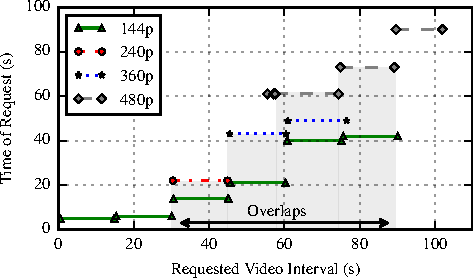
\includegraphics[width=0.9\linewidth]{figs/eg_request_schedule}%
\caption{Request schedule TODO: remake figure}
\label{fig:request_schedule}%
\end{figure}

\cite{sieber16sacrificing,sieber15costaggressive}